En esta sección mostraremos el Diagrama de interrelación de documentos(DID) creado a partir del DER mostrado en la sección
anterior.

\begin{figure}[H]
  \centering
    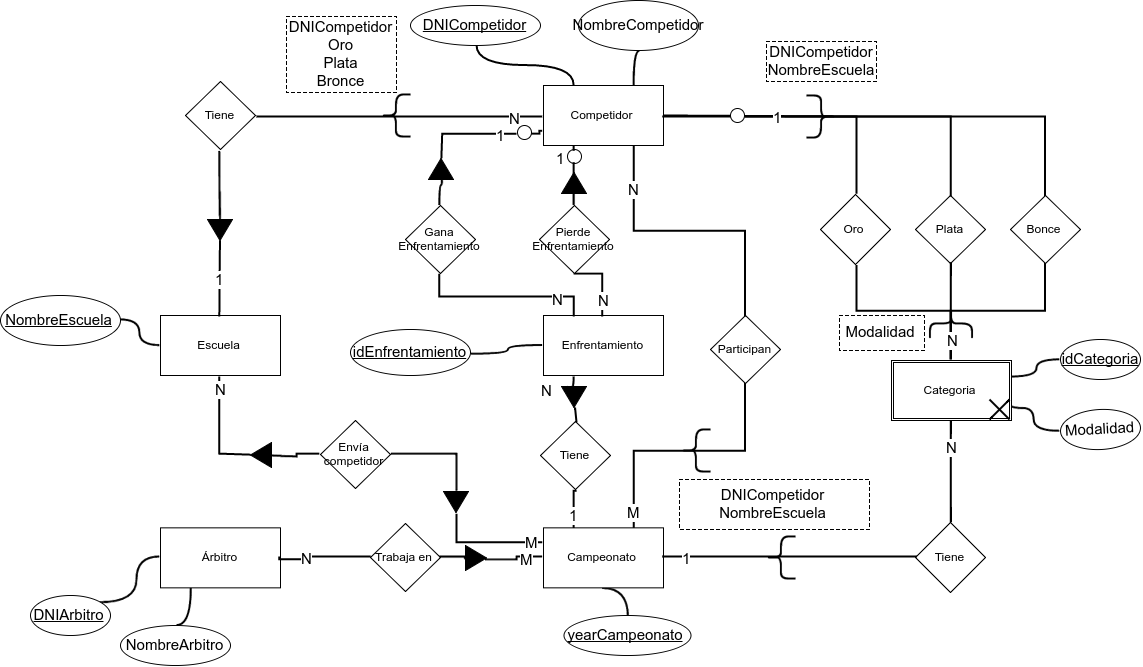
\includegraphics[scale=0.4]{imagenes/DID.png}
  \caption{Diagrama entidad relación}
\end{figure}

A continuación mostraremos la forma en la que se resolvieron las consultas pedidas y como las decisiones tomadas las
optimizan.

\subsection{Consultas}
\begin{enumerate}
\item Se nos pide la cantidad de enfrentamientos ganados por competidor para un campeonato dado. Se nos da como parámetro
el año del campeonato. Para resolver la consulta, recorremos todos los competidores en ListaCompetidores del campeonato.
Contamos la cantidad de enfrentamientos ganados usando EnfrentamientosGanados. Podemos realizar esta consulta con este
grado de optimización en el cual no buscamos otros documentos y nos basta solamente usar el documento de Campeonato. Esto
se debe a que Campeonato tiene embebido parcialmente a los documentos de Competidores que participan en él. A su vez, los
Competidores tienen referenciados a los enfrentamientos que ganaron y perdieron. El embebido parcial es sobre el
DNICompetidor, para buscar cada competidor, y sobre EnfrentamientosGanados para poder contar la cantidad de victorias.

\item La cantidad de medallas por nombre de escuela en toda la historia. Se nos da el NombreEscuela, que es la clave primaria de Escuela.
Buscamos por este nombre hasta posicionarnos en la escuela pedida. Recorro la ListaCompetidores. Para cada competidor, realizo la suma de las medallas de los
tres tipos(oro, plata y bronce). Existen dos procesos en esta consulta. El primero es la búsqueda en el documento Escuela
usando el NombreEscuela. Esta consulta es inevitable dado que necesitamos de la entrada de la escuela pedida para obtener
los demás datos. La segunda parte consiste en realizar la suma de todas las medallas de todas las entradas de
competidores. Esta segunda parte se beneficia del hecho de que posee ListaCompetidores gracias a que se tomo la decisión
embebido parcialmente a los competidores en el documento Escuela.

\item Para cada escuela, el campeonato donde ganó más medalla. Para realizar la consulta recorro el conjunto de
escuelas y, para cada una, recorro los campeonatos referenciados en ListaCampeonatos. Dentro de cada
campeonato recorro la ListaCategorias buscando a los ganadores de los distintos tipos de medallas cuyo NombreEscuela
coincida con el que estoy usando y sumo la cantidad de medallas de cada tipo. Me quedo con el campeonato con mayor
cantidad de medallas. Esta consulta fue optimizada gracias a que los documentos Escuela tienen referencia a los documentos
Campeonato(por su año). Se accede a cada documento campeonato y se utiliza que estos tienen embebidos a los Competidores.

\item Los árbitros que participaron en al menos 4 campeonatos. La consulta se realiza recorriendo los documentos
de Árbitro contando los Campeonatos usando ListaCampeonatos. Finalmente nos quedamos con los árbitros donde la ListaCampeonatos
tiene, al menos, 4 campeonatos distintos. Para cada árbitro, el proceso se resume en contar los campeonatos en la lista.
Podemos realizar esto gracias a ListaCampeonatos, la cual obtenemos gracias a que el documento Arbitro posee referencias
al documento Campeonato.

\item Las escuelas que han presentado el mayor número de competidores en cada campeonato. Recorro el conjunto de documentos
Campeonato y para cada uno recorro su ListaEscuela y para cada NombreEscuela veo cuales de la ListaCompetidores son de esa
Escuela. La consulta es optimizada debido a que los Campeonatos tienen referencias de los documentos Escuela y embebido parcialmente
a Competidor por el atributo NombreEscuela. Con lo cual, no se necesita acceder a otro documento que no sean todas las
entradas de Campeonatos. Esto último es necesario ya que necesitamos información de todos.

\item Obtener los competidores que más medallas obtuvieron por modalidad. Por cada entrada de el documento Competidor,
cuento las medallas de cada tipo que coinciden con la modalidad pedida. Después me quedo con los competidores que más entradas
totales tienen. Esta consulta se beneficia de que el Competidor tiene embebido parcialmente el documento Categoría por el
atributo Modalidad y por los ganadores de las tres medallas. Por lo tanto, no es necesario acceder a ningún otro documento
que no sea Competidor.

\end{enumerate}
